\chapter{Wstęp}
\section{Temat i cel projektu}
Tematem projektu jest, ''System do zarządzania biblioteką wykorzystujący głosowy interfejs użytkownika'', w ramach, którego został opracowany wielomodalny interfejs użytkownika służący do obsługi biblioteki.\ Celem projektu było zbadanie i wykorzystanie możliwości WebSpeechApi~\cite{WebSpeechApi} w celu umożliwienia poruszania się na stronie internetowej w sposób tradycyjny (klikany) oraz głosowy.

\section{Założenia techniczne}

\begin{table}[H]
    \centering
    \captionsource{Technologie wykorzystywane w projekcie}{Opracowanie własne}
    \label{tab:tech}
    \begin{tabular}{|r|r|} \hline
       \textbf{Typ aplikacji} & Aplikacja internetowe \\ \hline
       \textbf{Język oprogramowania} & PHP~7.4~\cite{Php2023} \\ \hline
       \textbf{Baza danych} & PostgreSql~\cite{Pos023} \\ \hline
        \multirow{3}*{\textbf{Wykorzystane biblioteki}} & Symfony~5.4~\cite{Sym2023} \\
        \cline{2-2}
        & WebSpeechApi~\cite{WebSpeechApi} \\
        \cline{2-2}
        & Bootstrap~\cite{Bootstrap2023} \\ \hline
    \end{tabular}
\end{table}

W \refsource{tabeli}{tab:tech} opisano założenia techniczne aplikacji internetowej, jakie przyjęto w trakcie wykonywania aplikacji.\ Załozenia opisują wybrany język oraz technologie, jakie posłużyły w utworzeniu całej aplikacji.\ Przepływ informacji pokazywanych Klientowi został przedstawiony na \refsource{diagramie}{fig:diag}.

\begin{figure}[H]
    \centering
    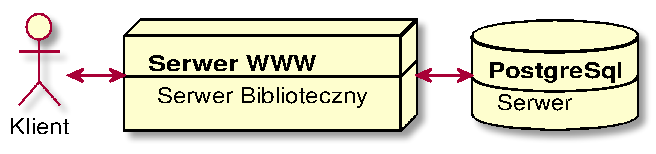
\includegraphics[width=0.5\textwidth]{./images/tech_diag}
    \label{fig:diag}
    \captionsource{Schemat systemu wraz z komunikacją}{Opracowanie własne}
\end{figure}

Cały system składa się serwera aplikacji internetowej napisanej w języku PHP~7.4~\cite{Php2023} , wykorzystującej framework Symfony~5.4~\cite{Sym2023} oraz z serwera bazodanowego wykorzystującego PostgreSQL~10~\cite{Pos023}. Do komunikacji głosowej aplikacja wykorzystuje WebSpeechApi~\cite{WebSpeechApi}, która umożliwia rozpoznawanie języka polskiego i przetwarzanie go na tekst.\ Dzięki czemu jest możliwość sterowania aplikacją przy pomocy głosu.